% !TeX root = ../../Skript.tex
\cohead{\Large\textbf{Momentane Änderungsrate}}
\fakesubsection{Momentane Änderungsrate an einzelnen Punkten}
Grafisch kann man die momentane Änderungsrate bzw. Steigung bzw. Ableitung einer Funktion an einer Stelle \(x_0\) abschätzen, indem man die Tangente einzeichnet und ihre Steigung bestimmt. Mathematisch bestimmt man die mittlere Änderungsrate mit Hilfe eines Steigungsdreiecks und schiebt dann die beiden Ecken, die auf der Funktion liegen auf einen Punkt zusammen:
\begin{tcolorbox}
	Berechnen der Ableitung:

	\(\makebox[\linewidth]{\textcolor{loestc}{\(f'(x_0)=\lim\limits_{h\to 0}\frac{f(x_0+h)-f(x_0)}{h}\)}}\)
\end{tcolorbox}
Den obigen Ausdruck nennt man Differentialquotient. Die Größe \(h\) entspricht der Breite des Steigungsdreiecks. Das \(lim\)-Zeichen (gesprochen Limes) steht für den Grenzwert. Wir lassen \(h\) immer näher gegen \(0\) gehen. Grob vereinfacht (und streng genommen falsch) wollen wir für \(h\) den Wert \(0\) einsetzen. Dann würden wir aber durch \(0\) teilen, was nicht definiert ist. Jedoch kann man den Bruch umformen bis man für \(h\) tatsächlich \(0\) einsetzen kann. Betrachten wir als Bsp. die Steigung von \(f(x)=x^2\) an der Stelle \(x_0=1\):

\begin{minipage}{\textwidth}
	\adjustbox{valign=t, padding = 0ex 0ex 2ex 0ex}{\begin{minipage}{0.4\textwidth-2ex}
		\centering\includegraphics[width=\textwidth]{\ableitung/pics/mom1\iftoggle{ausfuellen}{}{_empty}.png}
	\end{minipage}}%
	\adjustbox{valign=t}{\begin{minipage}{0.6\textwidth}
		\textcolor{loes}{Zeichnet man die Tangente an der Stelle \(x_0=1\) ein, so scheint die Steigung und damit die Ableitung den Wert 2 zu haben: \(f'(1)=2\)}

		\begin{align*}
			\textcolor{loes}{f'(1)}&\textcolor{loes}{=\lim\limits_{h\to 0}\frac{f(1+h)-f(1)}{h}=\lim\limits_{h\to 0}\frac{(1+h)^2-1^2}{h}}\\
			&\textcolor{loes}{=\lim\limits_{h\to 0}\frac{1+2h+h^2-1}{h}=\lim\limits_{h\to 0}\frac{2h+h^2}{h}}\\
			&\textcolor{loes}{=\lim\limits_{h\to 0}\frac{2+h}{1}=\lim\limits_{h\to 0}2+h=2}
		\end{align*}
	\end{minipage}}%
\end{minipage}

\medskip

Mit Hilfe des Differentialquotienten kann man also die Werte der Ableitung exakt berechnen. Dazu schreibt man den Quotienten aus und formt den Bruch dann so lange um bis man für \(h\) den Wert \(0\) einsetzen kann ohne, dass man durch \(0\) teilen würde.

Bestimmen wir nun noch die Ableitung von \(x^2\) an der Stelle \(x_0=-0,5\):
\begin{align*}
	\textcolor{loes}{f'(-0,5)}&\textcolor{loes}{=\lim\limits_{h\to 0}\frac{f(-0,5+h)-f(-0,5)}{h}=\lim\limits_{h\to 0}\frac{(-0,5+h)^2-(-0,5)^2}{h}}\\
	&\textcolor{loes}{=\lim\limits_{h\to 0}\frac{0,25-h+h^2-0,25}{h}=\lim\limits_{h\to 0}\frac{-h+h^2}{h}}\\
	&\textcolor{loes}{=\lim\limits_{h\to 0}\frac{-1+h}{1}=\lim\limits_{h\to 0}-1+h=-1}
\end{align*}
\newpage
%%%%%%%%%%%%%%%%%%%%%%%%%%%%%%%%%%%%%%%%%%%%%%%%%%%%%%%%%%%%%%%%%%%%%%%%%%%%%%%%%%%%%%%%%%%%%%%%%%%%%%
\begin{Exercise}[title={\raggedright Schätze jeweils die Ableitung an den Stellen -2 und 1 ab und berechne den Wert dann exakt.}, label=momA1]

    \begin{minipage}{\textwidth}
		\begin{minipage}{\textwidth}
			\adjustbox{valign=t, padding = 0ex 0ex 2ex 0ex}{\begin{minipage}{0.5\textwidth-2ex}
				\centering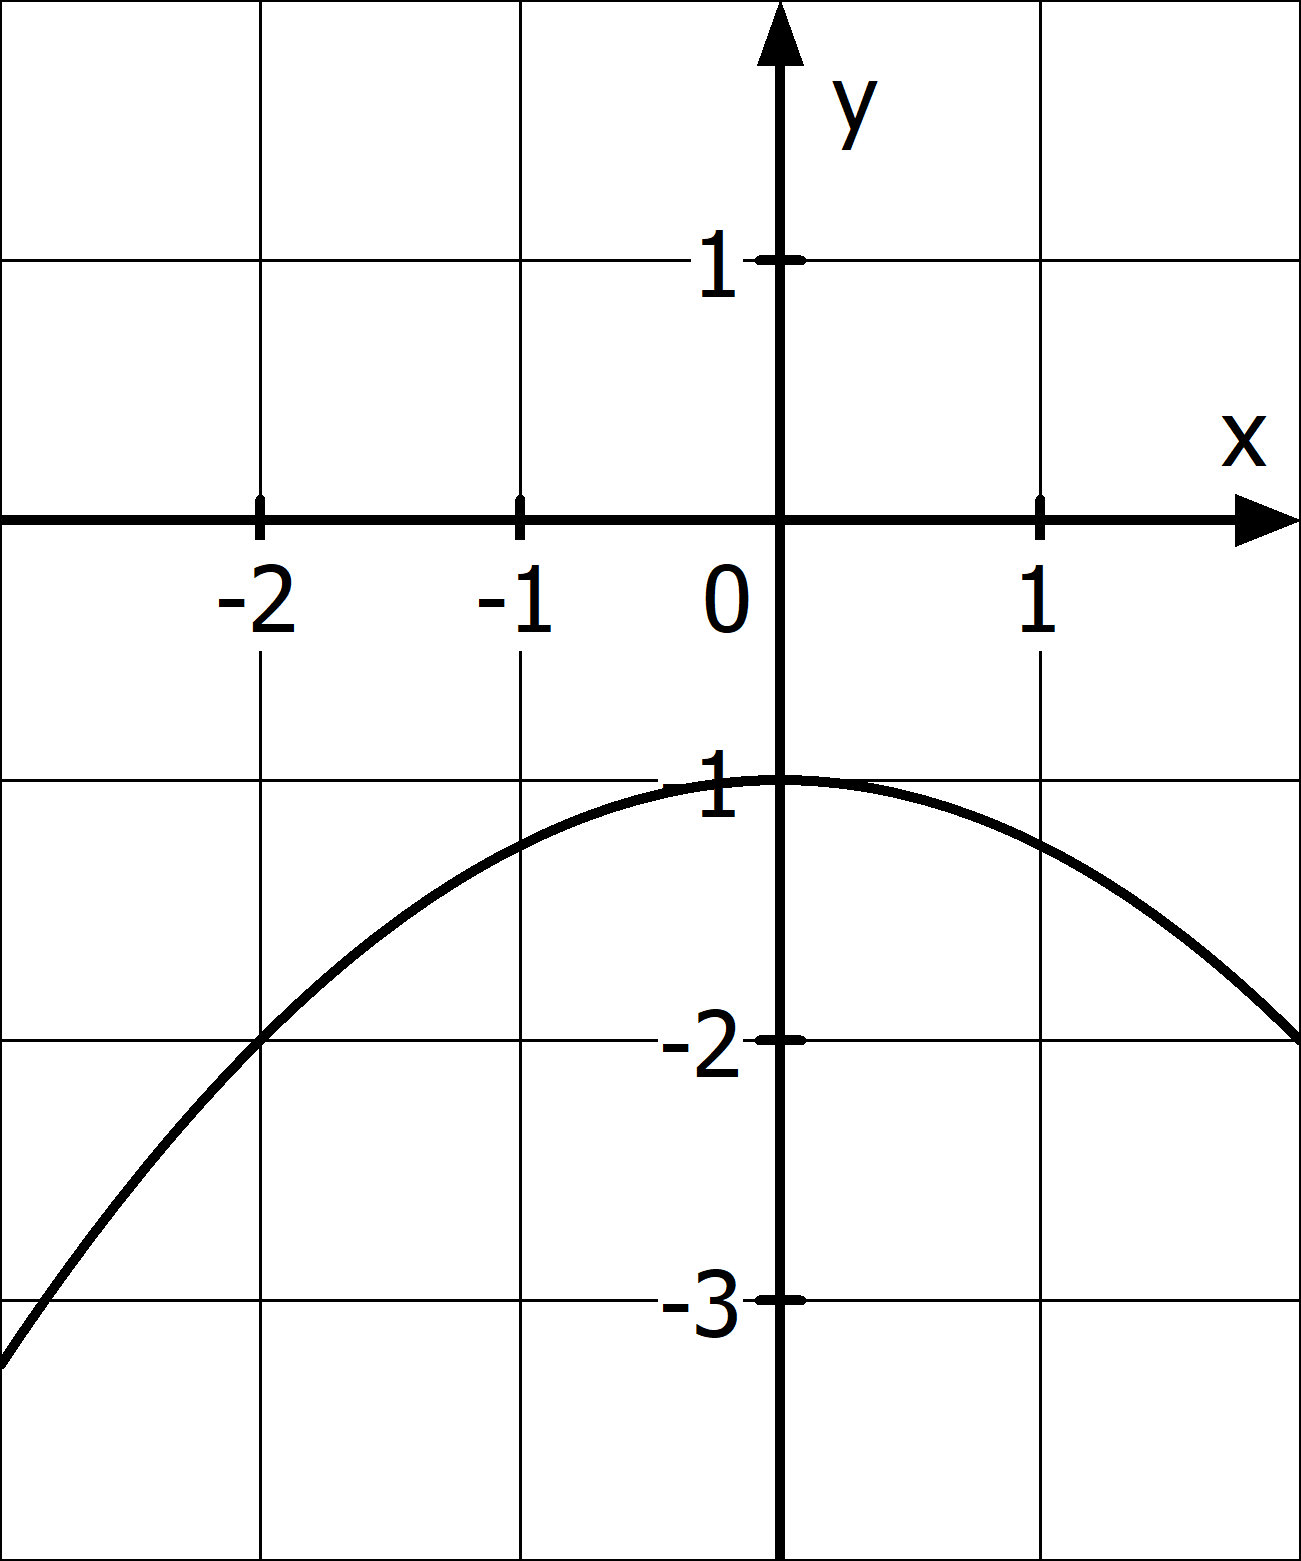
\includegraphics[width=\textwidth]{\ableitung/pics/momA1a.png}

				\(f(x)=-0,25x^2-1\)
			\end{minipage}}%
			\adjustbox{valign=t, padding = 2ex 0ex 0ex 0ex}{\begin{minipage}{0.5\textwidth-2ex}
				\centering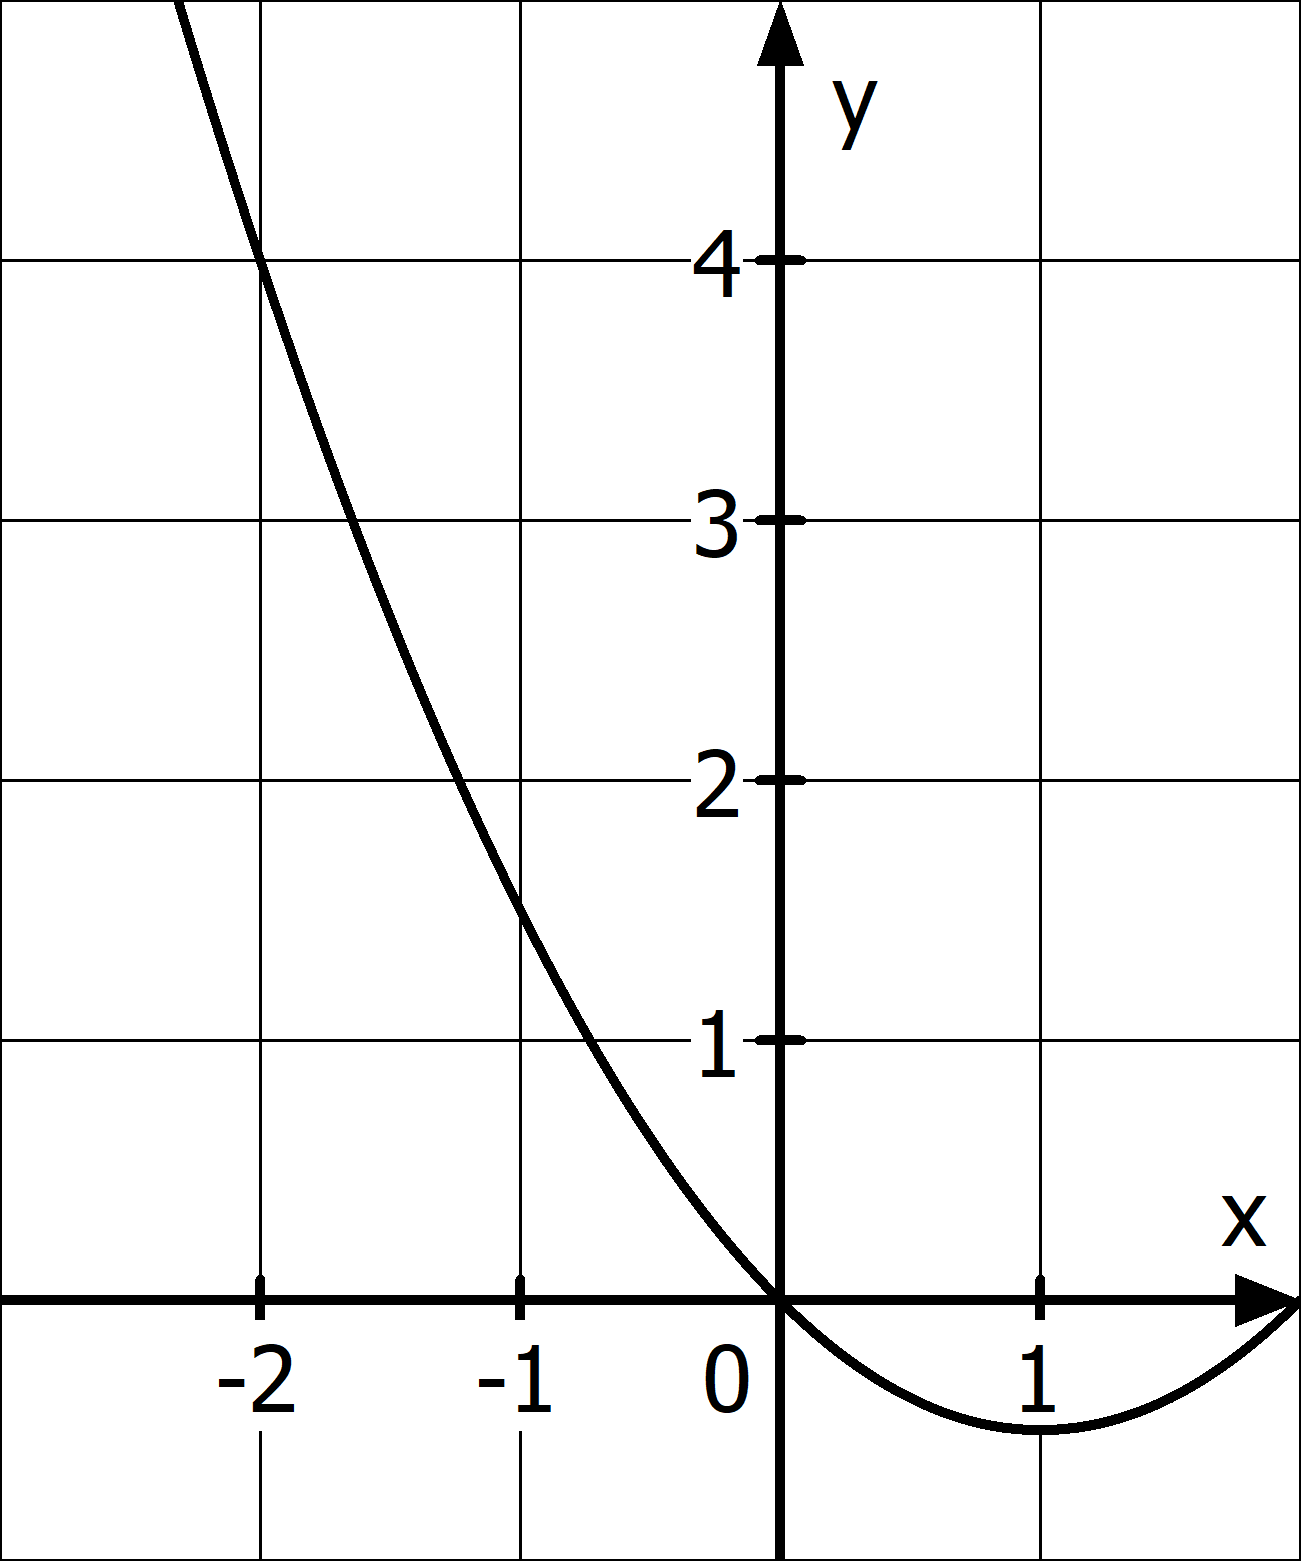
\includegraphics[width=\textwidth]{\ableitung/pics/momA1b.png}

				\(f(x)=0,5x^2-x\)
			\end{minipage}}%
		\end{minipage}%

        \medskip

		\begin{minipage}{\textwidth}
			\adjustbox{valign=t, padding = 0ex 0ex 2ex 0ex}{\begin{minipage}{0.5\textwidth-2ex}
				\centering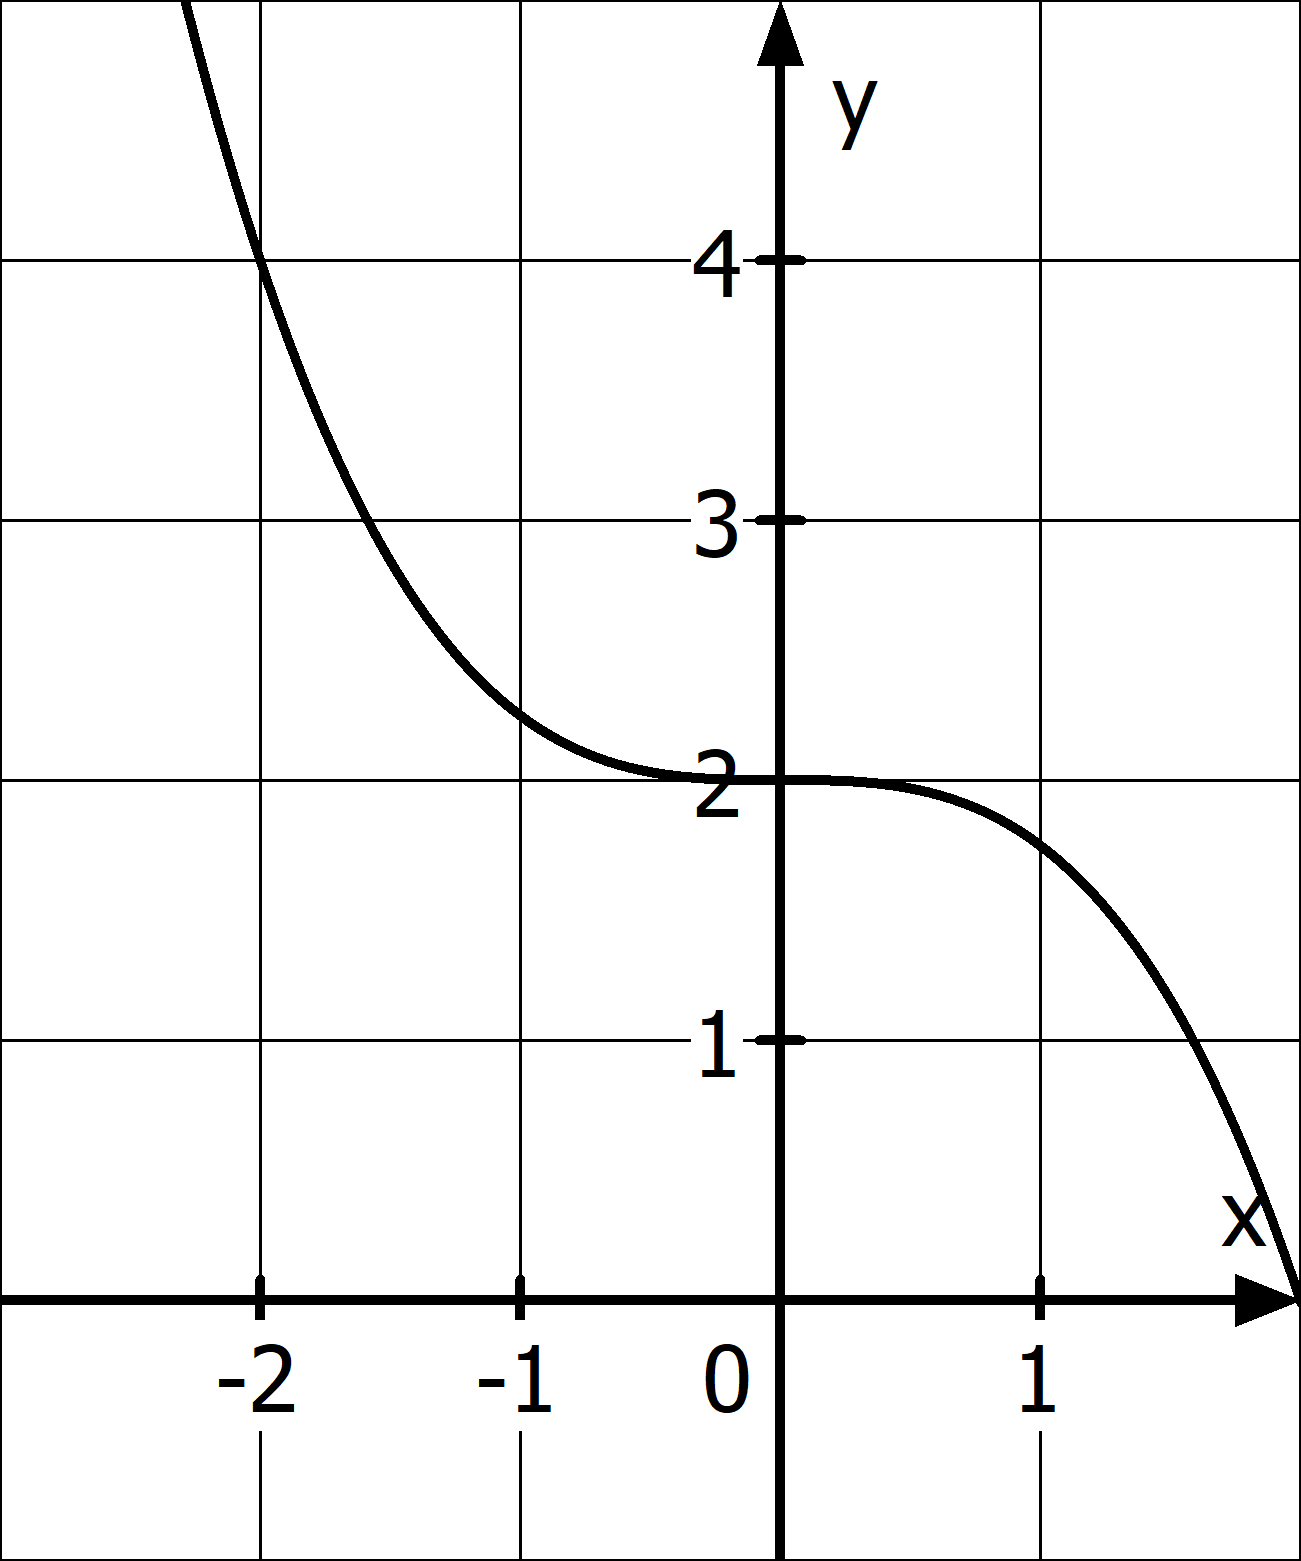
\includegraphics[width=\textwidth]{\ableitung/pics/momA1c.png}

				\(f(x)=-0,25x^3+2\)
			\end{minipage}}%
			\adjustbox{valign=t, padding = 2ex 0ex 0ex 0ex}{\begin{minipage}{0.5\textwidth-2ex}
				\centering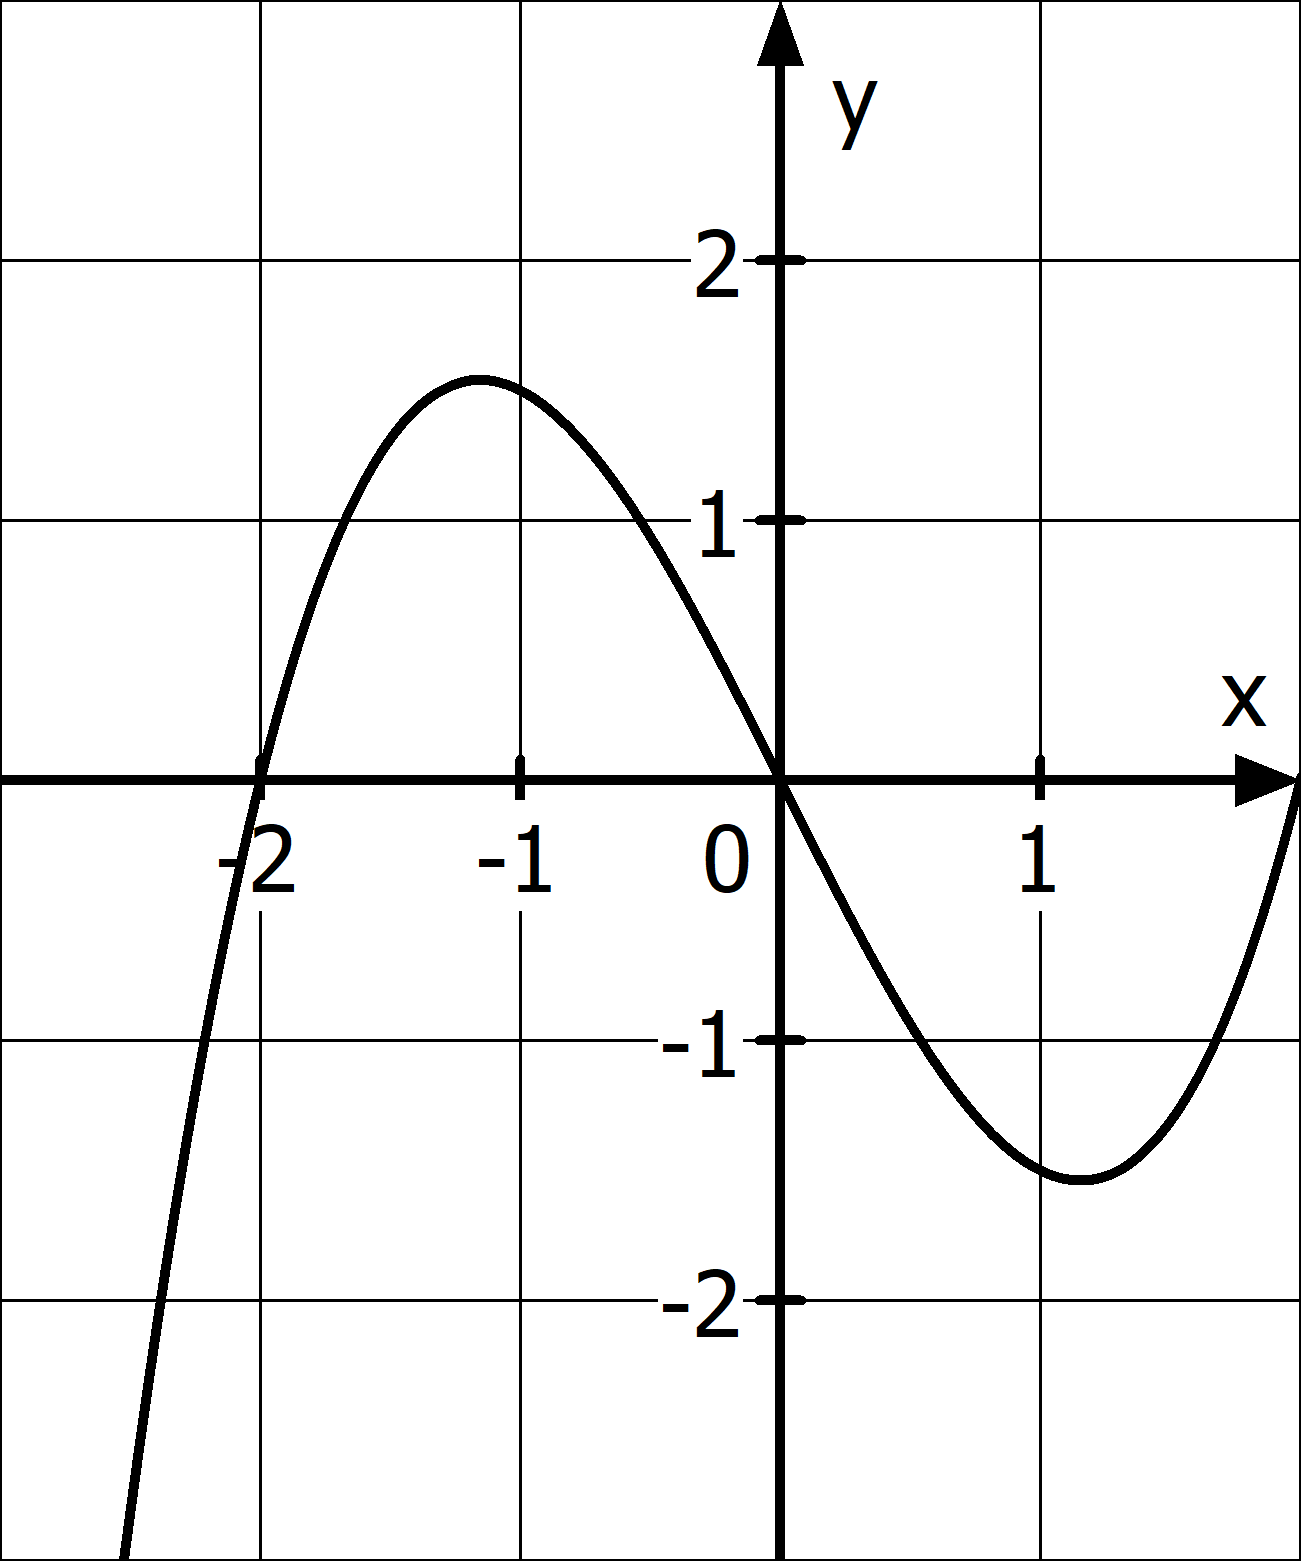
\includegraphics[width=\textwidth]{\ableitung/pics/momA1d.png}

				\(f(x)=0,5x^3-2x\)
			\end{minipage}}%
		\end{minipage}%
    \end{minipage}
\end{Exercise}
%%%%%%%%%%%%%%%%%%%%%%%%%%%%%%%%%%%%%%%%%
\begin{Answer}[ref=momA1]

	\begin{minipage}{\textwidth}
		\adjustbox{valign=t, padding = 0ex 0ex 2ex 0ex}{\begin{minipage}{0.35\textwidth}
			\centering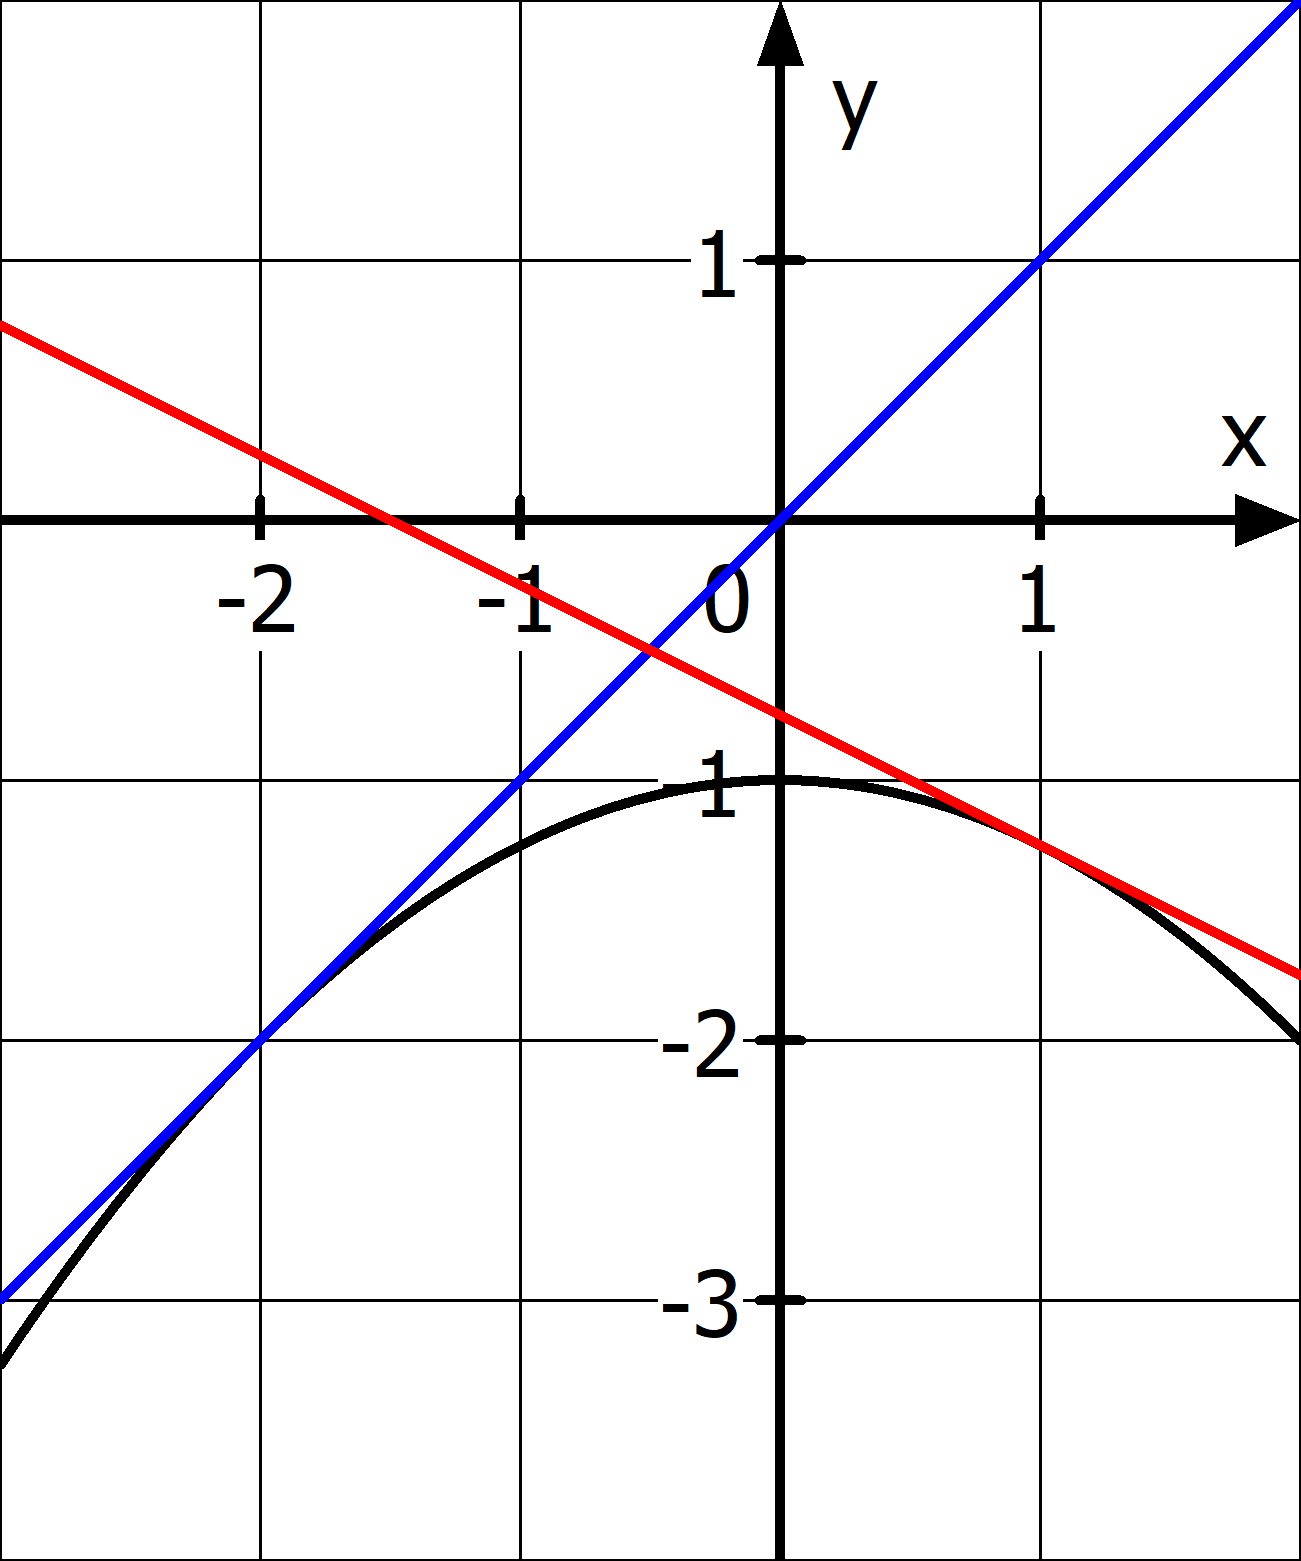
\includegraphics[width=\textwidth]{\ableitung/pics/momA1aL.png}\\
		\end{minipage}}%
		\adjustbox{valign=t}{\begin{minipage}{0.65\textwidth-2ex}
			\(f(x)=-0,25x^2-1\)

			Schätzung: \(f'(-2)\approx1\) und \(f'(1)\approx-0,5\)

			Berechnung:
			\begin{align*}
				f'(-2)&=\lim\limits_{h\to 0}\frac{f(-2+h)-f(-2)}{h}\\
				&=\lim\limits_{h\to 0}\frac{-0,25(-2+h)^2-1-(-0,25(-2)^2-1)}{h}\\
				&=\lim\limits_{h\to 0}1-0,25h=1\\
				f'(1)&=\lim\limits_{h\to 0}\frac{f(1+h)-f(1)}{h}\\
				&=\lim\limits_{h\to 0}\frac{-0,25(1+h)^2-1-(-0,25\cdot 1^2-1)}{h}\\
				&=\lim\limits_{h\to 0}-0,5-0,25h=-0,5
			\end{align*}
		\end{minipage}}%
	\end{minipage}

    \medskip

	\begin{minipage}{\textwidth}
		\adjustbox{valign=t, padding = 0ex 0ex 2ex 0ex}{\begin{minipage}{0.35\textwidth}
			\centering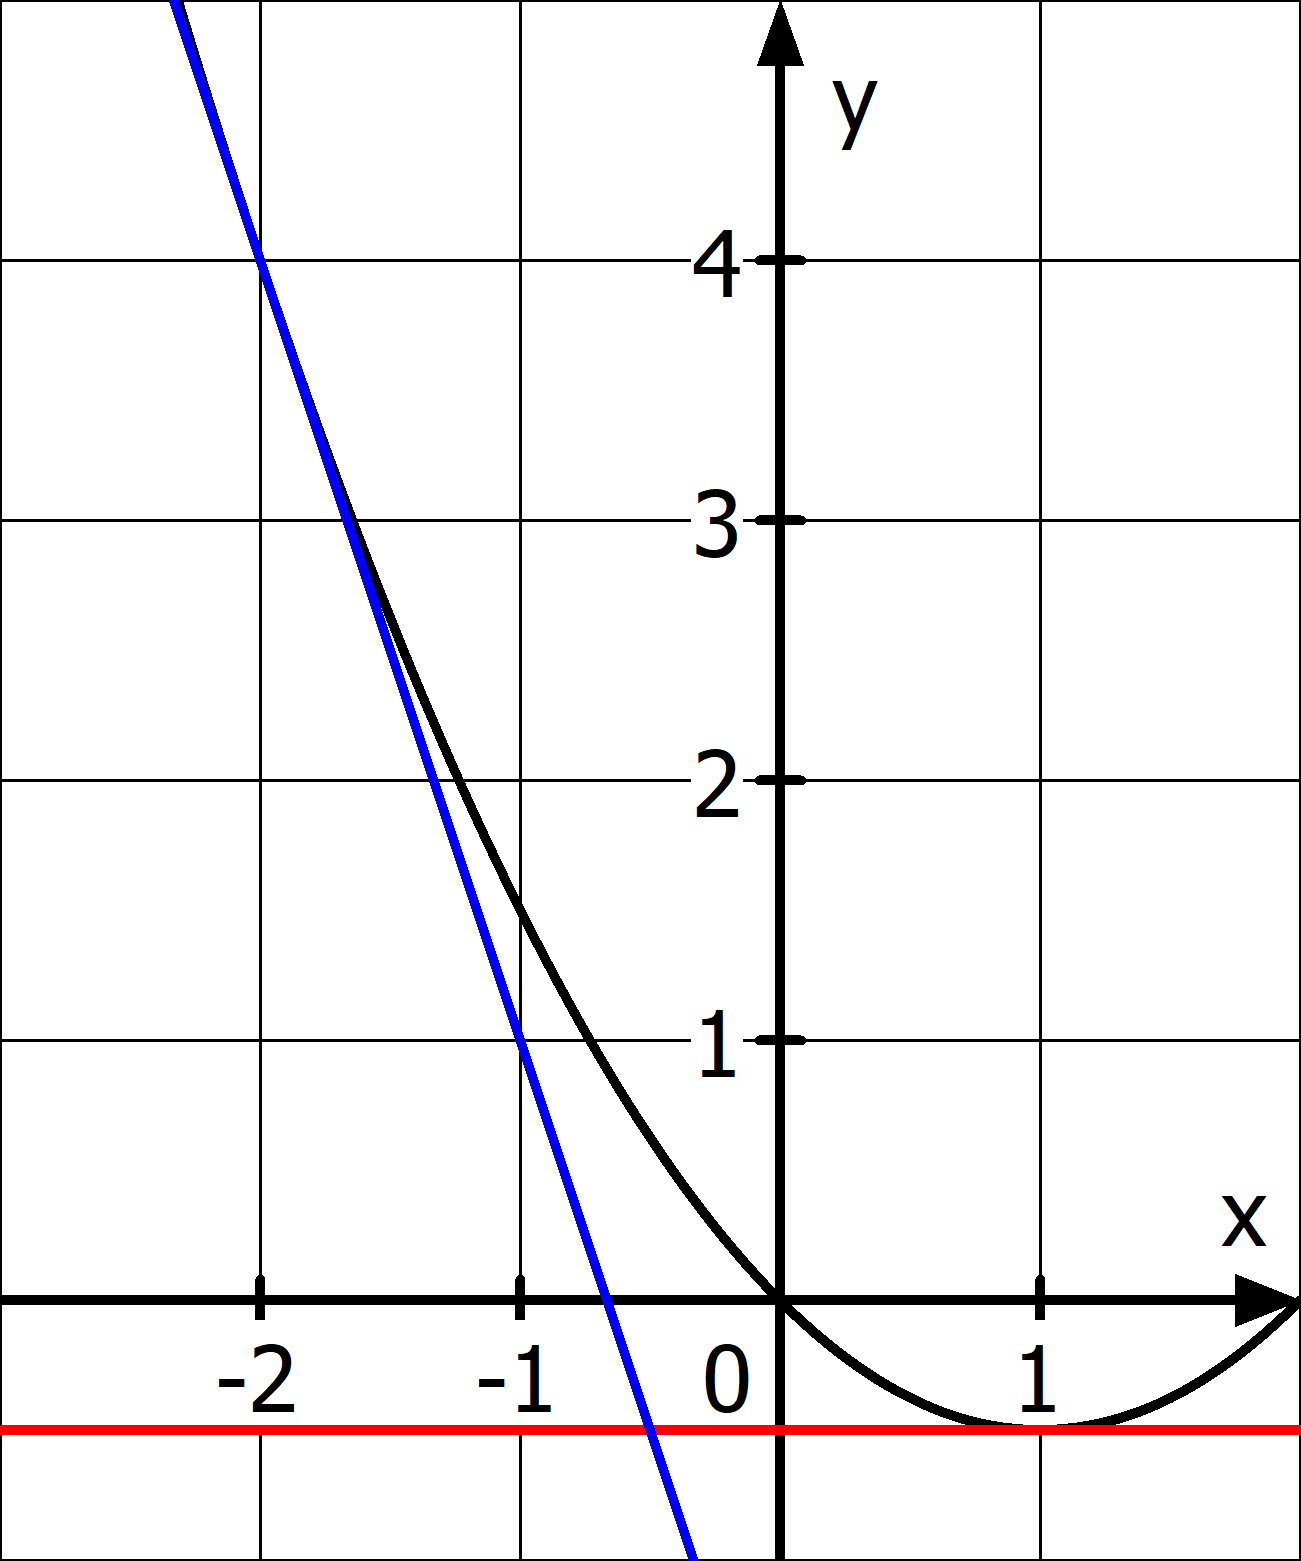
\includegraphics[width=\textwidth]{\ableitung/pics/momA1bL.png}
		\end{minipage}}%
		\adjustbox{valign=t}{\begin{minipage}{0.65\textwidth-2ex}
			\(f(x)=0,5x^2-x\)

			Schätzung: \(f'(-2)\approx-3\) und \(f'(1)\approx0\)

			Berechnung:
			\begin{align*}
				f'(-2)&=\lim\limits_{h\to 0}\frac{f(-2+h)-f(-2)}{h}\\
				=\lim\limits_{h\to 0}&\frac{0,5(-2+h)^2-(-2+h)-(0,5(-2)^2-(-2))}{h}\\
				&=\lim\limits_{h\to 0}-3+0,5h=-3\\
				f'(1)&=\lim\limits_{h\to 0}\frac{f(1+h)-f(1)}{h}\\
				&=\lim\limits_{h\to 0}\frac{0,5(1+h)^2-(1+h)-(0,5\cdot 1^2-1)}{h}\\
				&=\lim\limits_{h\to 0}0,5h=0
			\end{align*}
		\end{minipage}}%
	\end{minipage}

    \medskip

	\begin{minipage}{\textwidth}
		\adjustbox{valign=t, padding = 0ex 0ex 2ex 0ex}{\begin{minipage}{0.35\textwidth}
			\centering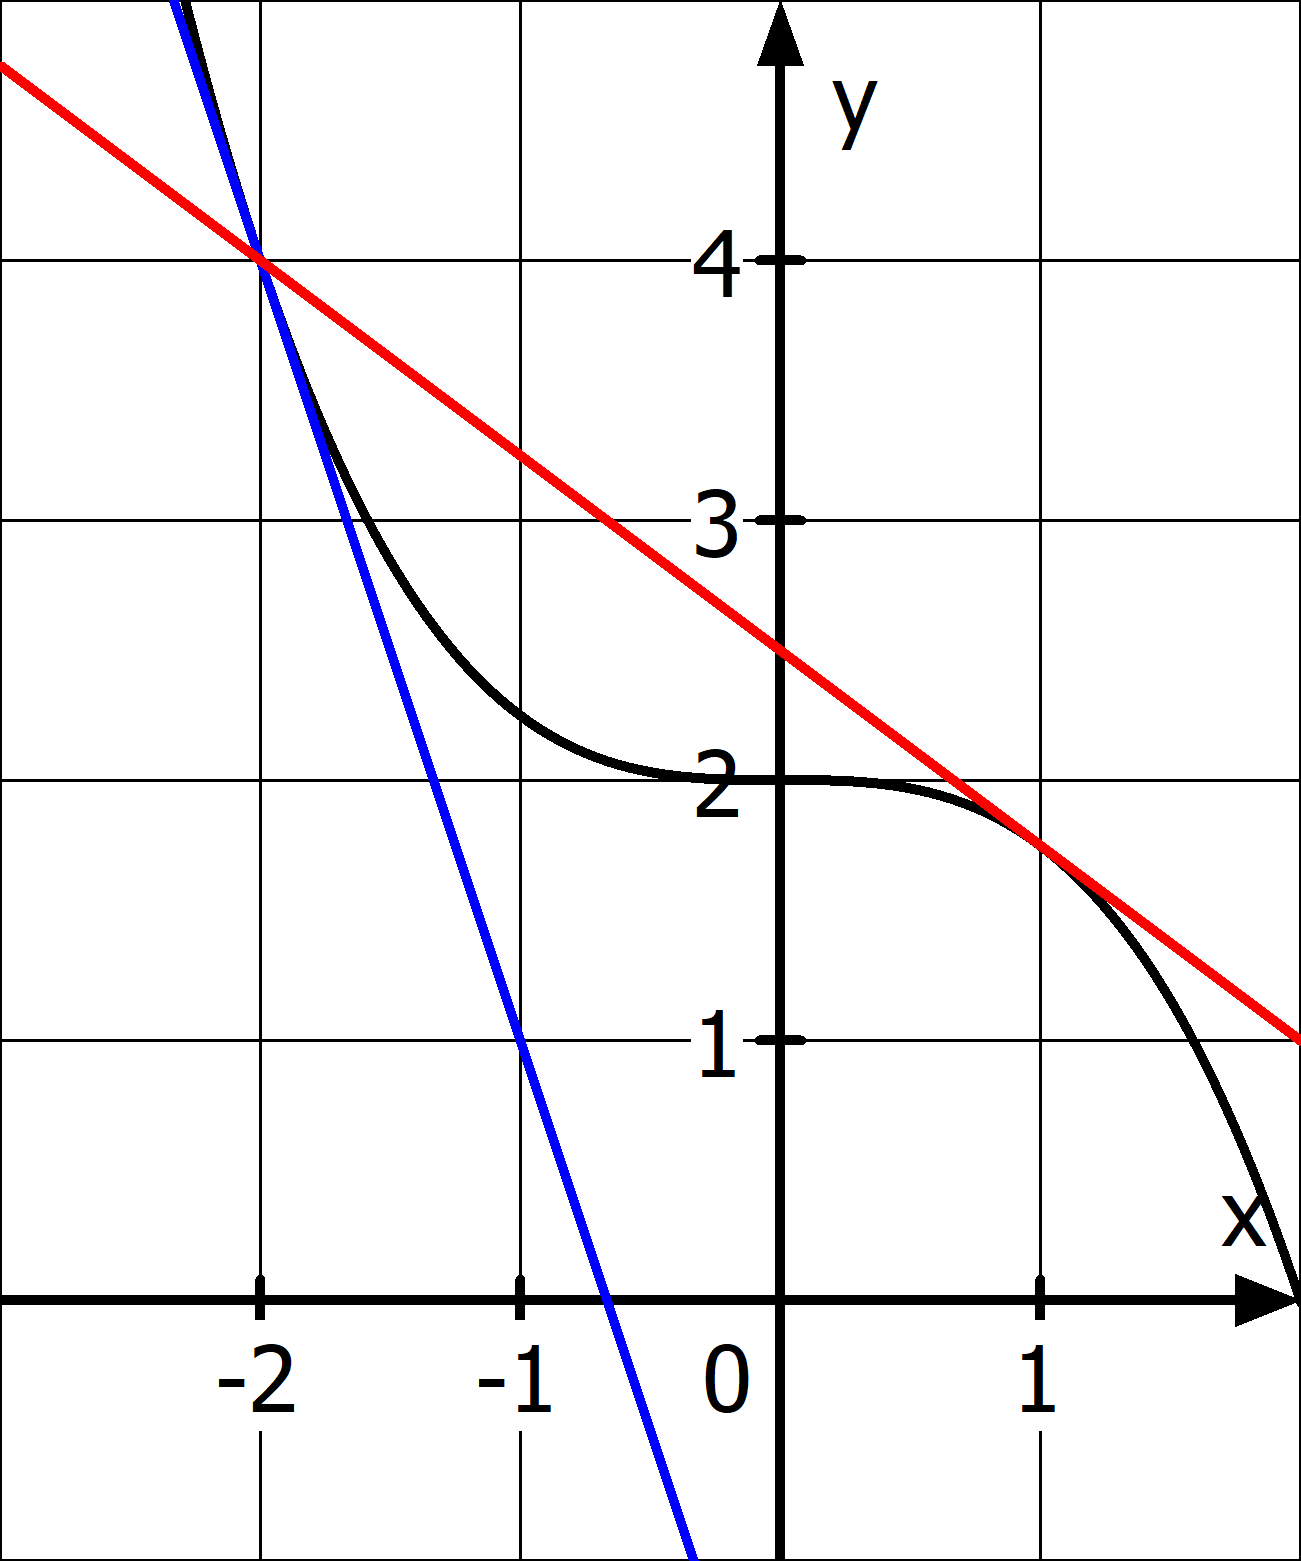
\includegraphics[width=\textwidth]{\ableitung/pics/momA1cL.png}
		\end{minipage}}%
		\adjustbox{valign=t}{\begin{minipage}{0.65\textwidth-2ex}
			\(f(x)=-0,25x^3+2\)

			Schätzung: \(f'(-2)\approx-3\) und \(f'(1)\approx-0,75\)

			Berechnung:
			\begin{align*}
				f'(-2)&=\lim\limits_{h\to 0}\frac{f(-2+h)-f(-2)}{h}\\
				&=\lim\limits_{h\to 0}\frac{-0,25(-2+h)^3+2-(-0,25(-2)^3+2)}{h}\\
				&=\lim\limits_{h\to 0}-3+1,5h-0,25h^2=-3\\
				f'(1)&=\lim\limits_{h\to 0}\frac{f(1+h)-f(1)}{h}\\
				&=\lim\limits_{h\to 0}\frac{-0,25(1+h)^3+2-(-0,25\cdot 1^3+2)}{h}\\
				&=\lim\limits_{h\to 0}-0,75-0,75h-0,25h^2=-0,75
			\end{align*}
		\end{minipage}}%
	\end{minipage}

    \medskip

	\begin{minipage}{\textwidth}
		\adjustbox{valign=t, padding = 0ex 0ex 2ex 0ex}{\begin{minipage}{0.35\textwidth}
			\centering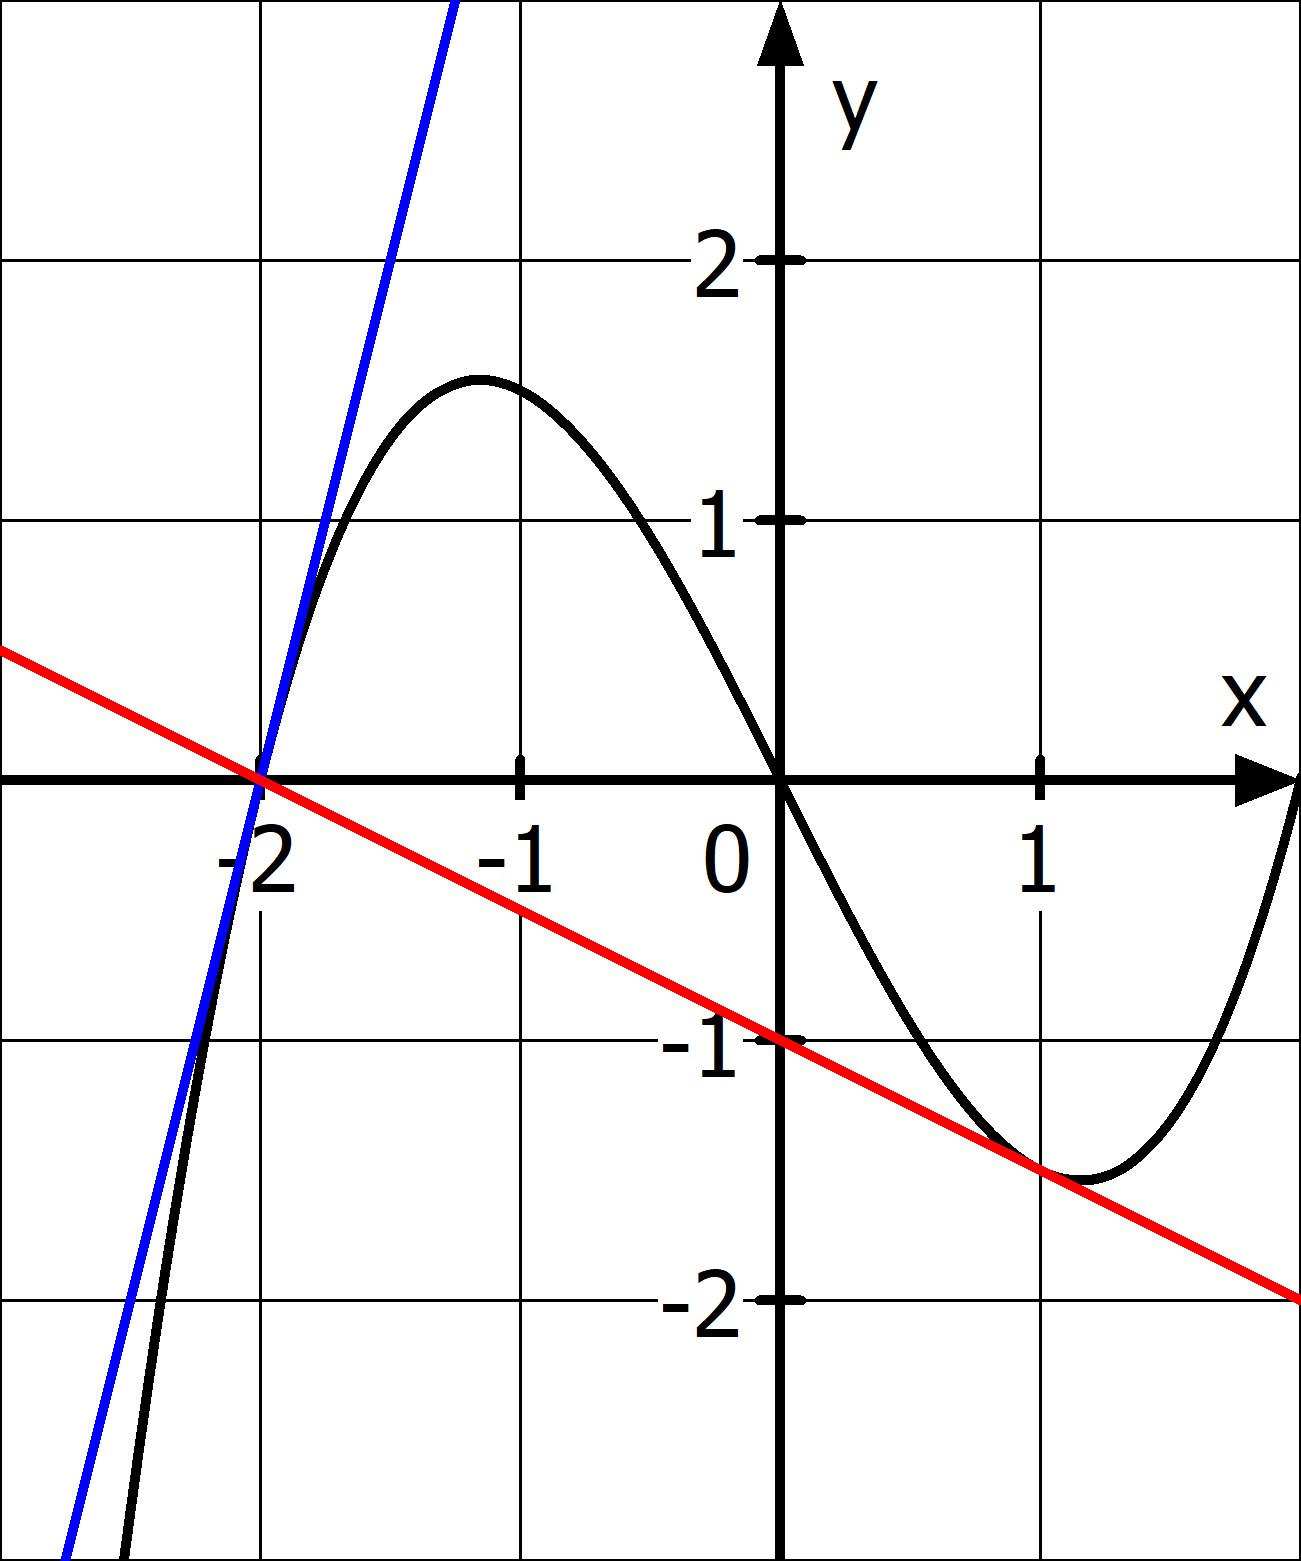
\includegraphics[width=\textwidth]{\ableitung/pics/momA1dL.png}
        \end{minipage}}%
		\adjustbox{valign=t}{\begin{minipage}{0.65\textwidth-2ex}
			\(f(x)=0,5x^3-2x\)

			Schätzung: \(f'(-2)\approx4\) und \(f'(1)\approx-0,5\)

			Berechnung:
			\begin{align*}
				f'(-2)&=\lim\limits_{h\to 0}\frac{f(-2+h)-f(-2)}{h}\\
				=\lim\limits_{h\to 0}&\frac{0,5(-2+h)^3-2(-2+h)-(0,5(-2)^3-2(-2))}{h}\\
				&=\lim\limits_{h\to 0}4-3h+0,5h^2=4\\
				f'(1)&=\lim\limits_{h\to 0}\frac{f(1+h)-f(1)}{h}\\
				&=\lim\limits_{h\to 0}\frac{0,5(1+h)^3-2(1+h)-(0,5\cdot 1^3-2\cdot 1)}{h}\\
				&=\lim\limits_{h\to 0}-0,5+1,5h+0,5h^2=-0,5
			\end{align*}
		\end{minipage}}%
	\end{minipage}
\end{Answer}